\chapter{Methods}

\section{Project Pipline}

The project pipeline contains 8 distinct phases that are shown in the figure~\ref{fig:pipline}. 
The pipeline begins by building the physical prototype of the robot. 
The second phase involved setting up the hardware and software required for the project, which included the initial introduction to the ROS 2 ecosystem. This phase involved learning and implementing foundational concepts necessary for the subsequent stages of the project. 
The third phase implements the ROS2 installations and tests its functionality by establishing a connection through two nodes, one running on the onboard computer and another on the control unit. 
The fourth phase carries out the development of the URDF file. 
The fifth phase vizualizes the URDF file in the RViz2 visualizer, and establishes the joint movement by using the package "joint state publisher." 
The sixth phase includes the simulation of the model within the Gazebo simulator. The DiffDrive plugin was used to control the simulation.
The seventh phase tested the remote control of the motor of the physical robot by using two ROS2 nodes: one listening for motor speed commands and one sending the motor speed commands. In the last phase, the three components—RViz, Gazebo, and drive node—were concatenated in a launch file and run simultaneously. 
This pipeline doesn't necessarily follow the structure of a best practice case, it shows how this project was built. 

\begin{figure}[h]
    \centering
    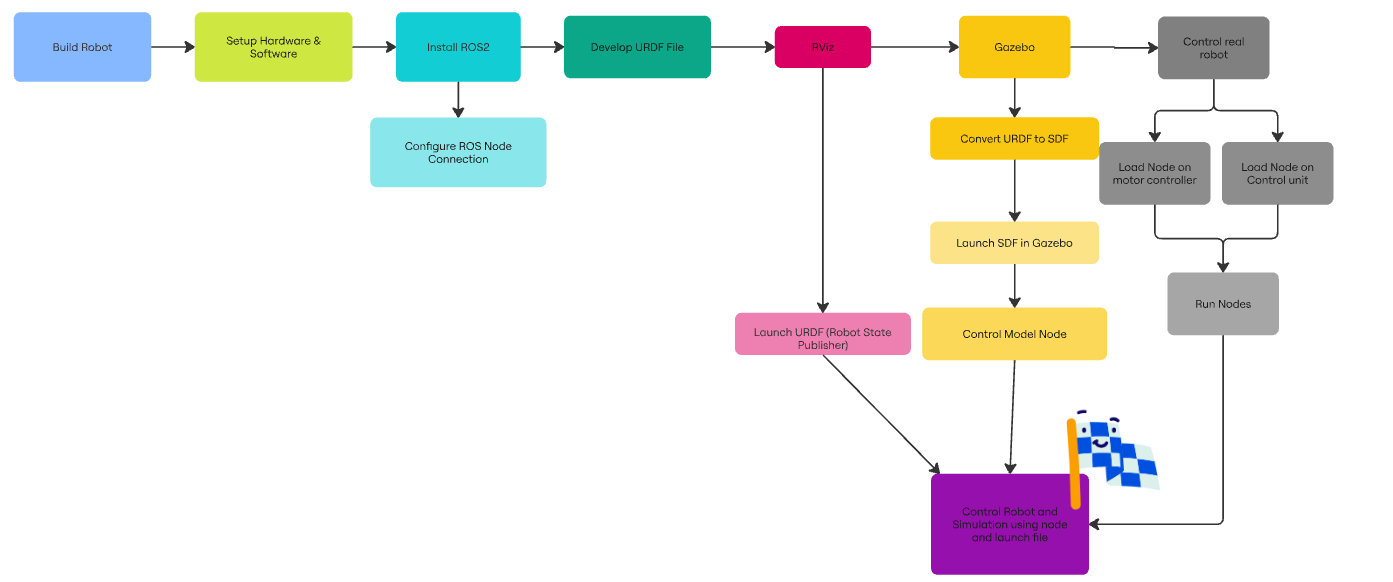
\includegraphics[width=0.9\textwidth]{Figures/project_pipline.png}
    \caption{Project Pipline}
    \label{fig:pipline}
\end{figure}
\autocite{openroboticsUrdfROSWiki}

\newpage
\section{Robot parts}

%% CG: check for repetetive phasing. 

The core elements may differ for different robot types, for this project, the core elements which were used to control the robot were the following: 

\begin{enumerate}
    \item motors
    \item power stations
    \item the motor drive
    \item the motor drive
    \item onboard computer
\end{enumerate}

The motors are the basic components which were used to give the robot the ability to move. In order to run the motors a power station which provides the appropriate voltage was included. By supplying the motors with electricity a basic movement of the motor could be achieved. 
To change the speed or direction and control them remotely, the robot was utilised with a motor driver. The motor driver took a low voltage and low current signal, primarily in the form of pulse width modulation (PWM), from the controller and amplified it using the power supply, creating a higher voltage and current feed to drive the motor.
The PWM signal consisted of a series of fast pulses, where the averaged value over time determined the percentage of the total voltage supplied to the motor. This ratio of on-time to off-time, known as the duty cycle, was implemented to regulate motor operation.
The motor control used more practical input formats, such as target speed, to calculate the appropriate signal for the driver. The driver, in turn, amplified this signal and transmitted it to the motor. A communication layer, a serial connection, was established to link the onboard computer with the motor controller. This communication allowed the onboard computer to send target speeds to the motor control.
The onboard computer was equipped with ROS2. The key tasks of ROS2 were to calculate the target motor speeds and translate these into a protocol compatible with the motor controller.

\section{System Setup of computer hardware and Software}

There are various computer hardware and software configurations available for working with ROS2, ranging from using a virtual machine with a Linux Ubuntu operation system (OS), to running a Docker container with a selected ROS2 image that can be run on a Windows OS by using the WSL2 \autocite{dockerRosOfficialImage}, or directly installing ROS2 on computer hardware that has Ubuntu Linux installed.
 In this project, all the previously mentioned methods were explored. The detailed experience will be discussed in more detail in the results in the chapter ''Installation computer hardware and software''.

\subsection{ROS2 installation}

The next step included the installation of the ROS2 Rolling on both the control unit and edge device. A detailed description of the installation can be found the installation guide A2. For Ubuntu 24.04 LTS the ROS2 distribution Rolling Ridely or Jazzy Jalisco can be used. For this stage of the project, the Rolling Ridely distribution was used. The Rolling Ridely is the rolling development distribution, which means it continuously integrates the latest features, updates and improvements \autocite{openroboticsDistributionsROS2}. This also makes it more unstable than the Jazzy Jalisco, which introduces several complications, as will be discussed in a later chapter. To guarantee a stable model in the future, a distribution change will be necessary. 

\subsection{Network configuration}

The network structure can be set up in multiple ways and should be dependent on the requirements a project has. For this project, two existing networks—home and ZHAW—were planted to be utilized. 


\subsection{ROS2 Nodes}

The development of the project relied heavily on the usage and development of Nodes and the communication system between nodes and topics. The primary used node was the demo node talker/listener, it was used to test the communication between the control unit and the edge device. These six additional nodes were used within this project: 

\begin{itemize}
    \item \verb|robot_state_publisher|: Publishes the URDF model to the /robot\_description topic for visualization and simulation.
    \item \verb|joint_state_publisher|: Publishes the robot's joint states for visualizing movements in RViz2.
    \item \verb|rviz2|: Launches RViz2 with a predefined configuration to visualize the robot's state.
    \item \verb|ros_gz_sim|: Simulates the environment and robot model based on control commands.
    \item \verb|ros_gz_bridge|: Connects ROS 2 and Gazebo to enable communication for movement commands.
    \item \verb|cmd_vel_to_motor_command|: Converts /cmd\_vel commands into motor commands for the real robot and Gazebo.
\end{itemize}

In order for these six nodes to send and receive data from each other the following topics where used:

\begin{itemize}
    \item \verb|/robot_description|: Publishes the robot's URDF model for visualization in RViz2 and simulation in Gazebo.
    \item \verb|/joint_states|: Publishes the state of the robot's joints.
    \item \verb|/cmd_vel|: Sends velocity commands (linear and angular) to control the robot's movement.
    \item \verb|/motor_command|: Simulates the environment and robot model based on control commands.
    \item \verb|ros_gz_bridge|: Transmits motor-specific commands to the real robot's motor controller.
    \item \verb|/tf|: Publishes transformations for coordinate frames.
\end{itemize}



\section{Develop URDF File}

To create a digital twin, a robot description is required. This description contains all the information about the robot's physical characteristics and is stored in a URDF file. The structure of a URDF file follows a simple and repetitive pattern. At its core, it consists of a tree of links connected by joints. The links represent the robot's physical components, such as wheels, while the joints define the dynamic relationships between these components—for example, the rotation of a wheel relative to the robot's body.
When defining a joint, a specific type must be assigned. The available joint types are:

\begin{itemize}
    \item Revolute: Rotational motion with defined minimum and maximum angle limits.
    \item Continuous: Unlimited rotational motion, such as that of a wheel.
    \item Prismatic: Linear sliding motion with specified minimum and maximum position limits.
    \item Fixed: A rigid connection where the child link is immovably attached to the parent link, often used for "convenience" links.
\end{itemize} \autocite{newansDescribingRobotsURDF}

URDF files are written in XML, with their content represented as a series of nested tags. The primary tags used in this project include were robot tag, link tags and joint tags.

\subsection{The Robot tag}

The robot tag is the root element of the robot description file, encapsulating all other elements.  It is placed immediately following the XML declaration.  It is placed immediately following the XML declaration. \autocite{UrdfXMLROS}

\lstinputlisting[caption={Robot Tag code Example}, label={lst:robot_tag}]{Code/robot_tag.xml}

\subsection{Link tags}

The link tag defines a rigid body, specifying its visual features, and collision properties. \autocite{UrdfXMLROS}

\lstinputlisting[caption={Link Tag code Example}, label={lst:robot_tag}]{Code/link_tag.xml}

\subsection{Joint tags}

The joint tags describes the kinematics and dynamics of the joint, including its savety limits. It allways stands between a child link and it's parent link.\autocite{UrdfXMLROS} 

\lstinputlisting[caption={Joint Tag Code Example}, label={lst:robot_tag}]{Code/joint_tag.xml}

Additional tags such as sensor, model state or gazebo can be implementet. In this project, the URDF was used to establish a foundational understanding of how a robot description is configured. For the final simulation in Gazebo, the URDF file was converted into an SDF file, which is compatible with Gazebo and allows the model to be launched in the simulation environment.

\section{Launch URDF in RViz}
To visualize the URDF model, the ROS 2 visualization tool Rviz was used. There are several ways to launch a URDF in Rviz, but the simplest approach is to create a ROS 2 launch file. A ROS 2 launch file allows the simultaneous configuration and execution of multiple ROS 2 nodes. These launch files can be written in Python, XML, or YAML, depending on the project requirements. \autocite{CreatingLaunchFile}
For this project, a Python launch script was created. This script starts the following nodes.

\begin{itemize}
    \item The robot state publisher node, which publishes the robot's state to the tf2 transform tree,
    \item The joint state publisher gui node, enabling interactive control to move the robot's wheels, and
    \item The Rviz node, to visualize the URDF model in the Rviz interface.
\end{itemize}

\lstinputlisting[caption={Launch file structure}, label={lst:robot_tag}]{Code/launchfile.py}

\section{Gazebo}
The Gazebo simulator was utilized in this project to simulate the robot's behaviour and interactions within a virtual environment. Unlike RViz, Gazebo is not included as a default package in the ROS 2 Rolling installation. Similar to ROS 2, Gazebo is available in multiple distributions, each corresponding to a specific ROS 2 version. For the ROS 2 Rolling distribution, the Gazebo Ionic distribution must be installed. Detailed installation steps for Gazebo in the Rolling distribution are provided in Installation Guide A3. To launch the URDF file two options are given, the primary is to use the xacro program to create the URDF file. By doing so the necessary elements for simulation, such as link inertial properties, joint dynamics, and kinematic chains are included in the URDF file. The second option is to transition the URDF to the native Simulation Description Format (SDF) of gazebo. This option is especially recommended if additional Gazebo-specific features are needed for the model.

\section{Control the robot}

%% CG: In the methods you need to outline what you have done to understand how to control the robot and its digital twin. The actual implementation is part of the results section.

As a starting point to understand how the physical robot could be controlled remotely, a tutorial from the Articubot website was followed. This does not represent a scientific approach, however, it streamlined this part of the project significantly. The following key steps were recreated based on the tutorial:

\begin{itemize}
    \item Exploring the setup components and their interactions.
    \item Establishing an SSH connection from the control unit to the onboard computer using Visual Studio Remote.
    \item Utilizing the Arduino Extension within the Visual Studio Remote environment to upload scripts to the Arduino Mega (motor controller).
    \item Transmitting data, such as motor speed, from a node running on the control unit to the appropriate topic via messages, and receiving this data on a corresponding node running on the onboard computer.
\end{itemize}